\ifSTANDALONE
\section{Realisierung}
\fi
\ifEMBED
\subsection{Realisierung}
\fi 
    \ifSTANDALONE
    \subsection{Hardware} \label{ch:Hardware}
    \fi
    \ifEMBED
    \subsubsection{Hardware} \label{ch:Hardware}
    \fi
    Der L6480 besitzt, wie in \autoref{sec:L6480} beschrieben, eine 
    SPI-Schnittstelle. Über diese Schnittstelle soll der Steppertreiber die 
    Befehle des Freedomboards erhalten. Der Steppertreiberprint wird mit 
    Stiftleisten bestückt und kann so direkt auf das Freedomboard aufgesteckt 
    werden. Es wird so keine Kabelverbindung benötigt und die Elektronik 
    bleibt kompakt.
    \begin{figure}[h]
        \centering
        \begin{tikzpicture}
        \node[above right] (img) at (0,0) {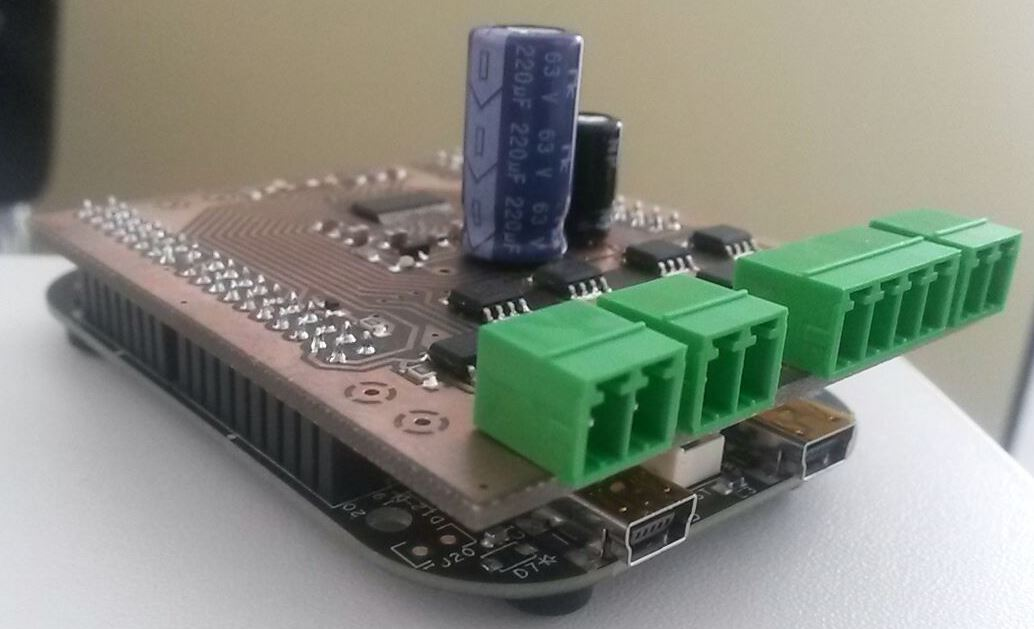
\includegraphics[width=8cm]{\EtPath/Bilder/hardware.jpg}};
        \draw[line width=1pt]
        (1.5, 0.75) node[below=1mm] {Freedom-Board}
        -- (2.7, 1);
        \fill (2.7,1) circle (2pt);
        \draw[line width=1pt]
        (2, 4) node[above=2mm] {Adapterprint}
        -- (2.7, 2);
        \fill (2.7,2) circle (2pt);
        \end{tikzpicture}
        \caption{Freedomboard und Steppertreiberprint}
        \label{fig:Steppertreiber}
    \end{figure}
    \newline
    Der Steppertreiberprint beinhaltet grundsätzlich den Treiber für den 
    Schrittmotor, realisiert mit dem Baustein L6480 und einer externen 
    H-Brücke aus N-FET. Zusätzlich sind Anschlüsse für andere Motoren (z.B.  
    BLDC-Motor) auf dem Print integiert. Im Folgenden wird die Entwicklung 
    dieses Adapterprints vogestellt. Ab Seite \pageref{sec:Schema} ist das 
    Schema der Schaltung und ab Seite \pageref{sec:PrintDesign} die 
    Beschreibung des Printdesigns zu finden. 
    % -----------------------------------------------------------------------------------
    \ifSTANDALONE
    \subsection{Schema} \label{sec:Schema}
    \fi
    \ifEMBED
    \subsubsection{Schema} \label{sec:Schema}
    \fi
    Als Motorencontroller wird der integrierte Schaltkreis L6480 von 
    STMicroelectronics verwendet. Dieser wird über eine SPI-Schnittstelle 
    angesteuert. Der l6480 bietet die Möglichkeit, Bewegungsprofile zu 
    konfigurieren. Die verschiedenen Betriebsarten werden im Kapitel 
    \ref{ch:Software} vorgestellt. Die H-Brücke wird extern mit N-FETs 
    realisiert. Die Beschaltung des L6480 kann aus dem Datenblatt 
    \cite{Datasheet:L6480} entnommen werden.\\\\ 
    Das revidierte Schema ist auf Seite \pageref{Schema} abgebildet.
    \\\\
    \textbf{Speisung}\\
    Es gibt zwei Möglichkeiten, wie das IC gespiesen werden kann: 
    \begin{itemize}
        \item Motorenspannung, interne Spannungsregler generieren die nötige 
            Gatespannung sowie die Logikspannung
        \item Externe Spannungsregler
    \end{itemize}
    Es wird die erste Möglichkeit, die Speisung mit nur der Motorenspannung 
    gewählt. Als Motorenspeisung ist ein Bereich von 10.5 \ldots 85\si{\volt} 
    zulässig. Bei eine Betriebsspannung von mehre als 25\si{\volt} sind MOSFET 
    mit einer höherenen Sperrspannung notwendig. Zusätzliche Spannungsregler 
    sind nicht notwendig. 
    \\\\
    \textbf{Motor supply voltage compensation}\\
    Der Motorcontoller bietet die Möglichkeit, Schwankungen der 
    Motorenspannung zu erkennen und so die Amplitude des PWM-Sinussignales am 
    Schrittmotor zu regeln. Dazu muss der Eingang ADCIN des Controllers 
    korrekt beschaltet werden. An diesem Analogeingang soll bei korrekter 
    Motorspannung 1/2 der Logikspannung anliegen. In diesem Fall bedeutet 
    dies, dass bei normaler Betriebsspannung 1.65\si{\volt} über dem 
    Widerstand R4 anliegen müssen. 
    \\\\
    \textbf{LED Speisung}\\
    Damit sofort ersichtlich ist, ob der Adapterprint gespiesen ist, wird eine 
    LED vorgesehen. Diese wird zwischen die Speisung über einen Vorwiderstand 
    an GND angeschlossen. Somit ist alles in Ordnung, falls die LED leuchtet.
    \\\\
    \textbf{LED Fehler}\\
    Der Motorencontroller kann so konfiguriert werden, dass verschiedene 
    Fehler angezeigt werden können. Dies beinhaltet zum Beispiel 
    Schrittverluste, Überstrom, Unterspannungserkennung oder Überhitzung des 
    Controllers. Dazu dient ein Open-Drain Pin $\overline{FLAG}$, welcher im 
    Fehlerfall auf GND zieht. Der Pin wird so beschaltet, dass eine LED den 
    Fehlerfall auch optisch sichtbar macht. 
    \\\\
    \textbf{Pinbelegung}\\
    Die Kommunikation mit dem Motorencontroller und die Ansteuerung des 
    Pneumatikventils wird mit dem Freedom-Board realisiert. 
    Die folgende Tabelle stellt die Schnittstelle zwischen dem Freedomboard 
    und den Anschlüssen auf dem Adapterprint dar. 
    \begin{table}[h!]
        \begin{zebralongtable}{p{3cm} p{2cm} p{1.5cm}}
             \rowcolor{gray}\textbf{Pin}                & \textbf{Stepper-board}   & \textbf{FRDM-KL25Z} \\           
            \textbf{IO L6480}\\ 
            %\cmidrule{1-1}
            $\overline{FLAG}$           & J2 Pin 2  & PTA13 \\ 
            $\overline{BUSY}$ / SYNC    & J1 Pin 2  & PTA1  \\ 
            $\overline{STBY / RESET}$   & J2 Pin 11 & PTA17 \\ 
            STCK                        & J2 Pin 9  & PTA16 \\ 
            %\cmidrule{1-1}
            \textbf{SPI L6480}          &           &       \\ 
            %\cmidrule{1-1}
            $\overline{CS}$             & J9 Pin 13 & PTE4  \\ 
            CK                          & J9 Pin 9  & PTE2  \\
            MOSI                        & J9 Pin 11 & PTE3  \\ 
            MISO                        & J2 Pin 20 & PTE1  \\ 
            \textbf{Pneumatik}\\ 
            Ventil                      & J2 Pin 18 & PTE0  \\ 
        \end{zebralongtable}
        \caption{Pinbelegung}
        \label{tab:Pinbelegung}
    \end{table} 
    \\
    \textbf{Zusätzliche Bestückung}\\
    Zusätzlich kann ein Bluetoothmodul bestückt werden. Weitere 
    Bestückungen...\\\\
    Es wird mit dem Tool Altium Designer gearbeitet. Das überarbeitete Schema 
    des Steppertreiberprints ist auf der Seite \pageref{Schema} zu finden. 
    %*****************************************************
    % Schema Stepperboard                                %
    %*****************************************************
    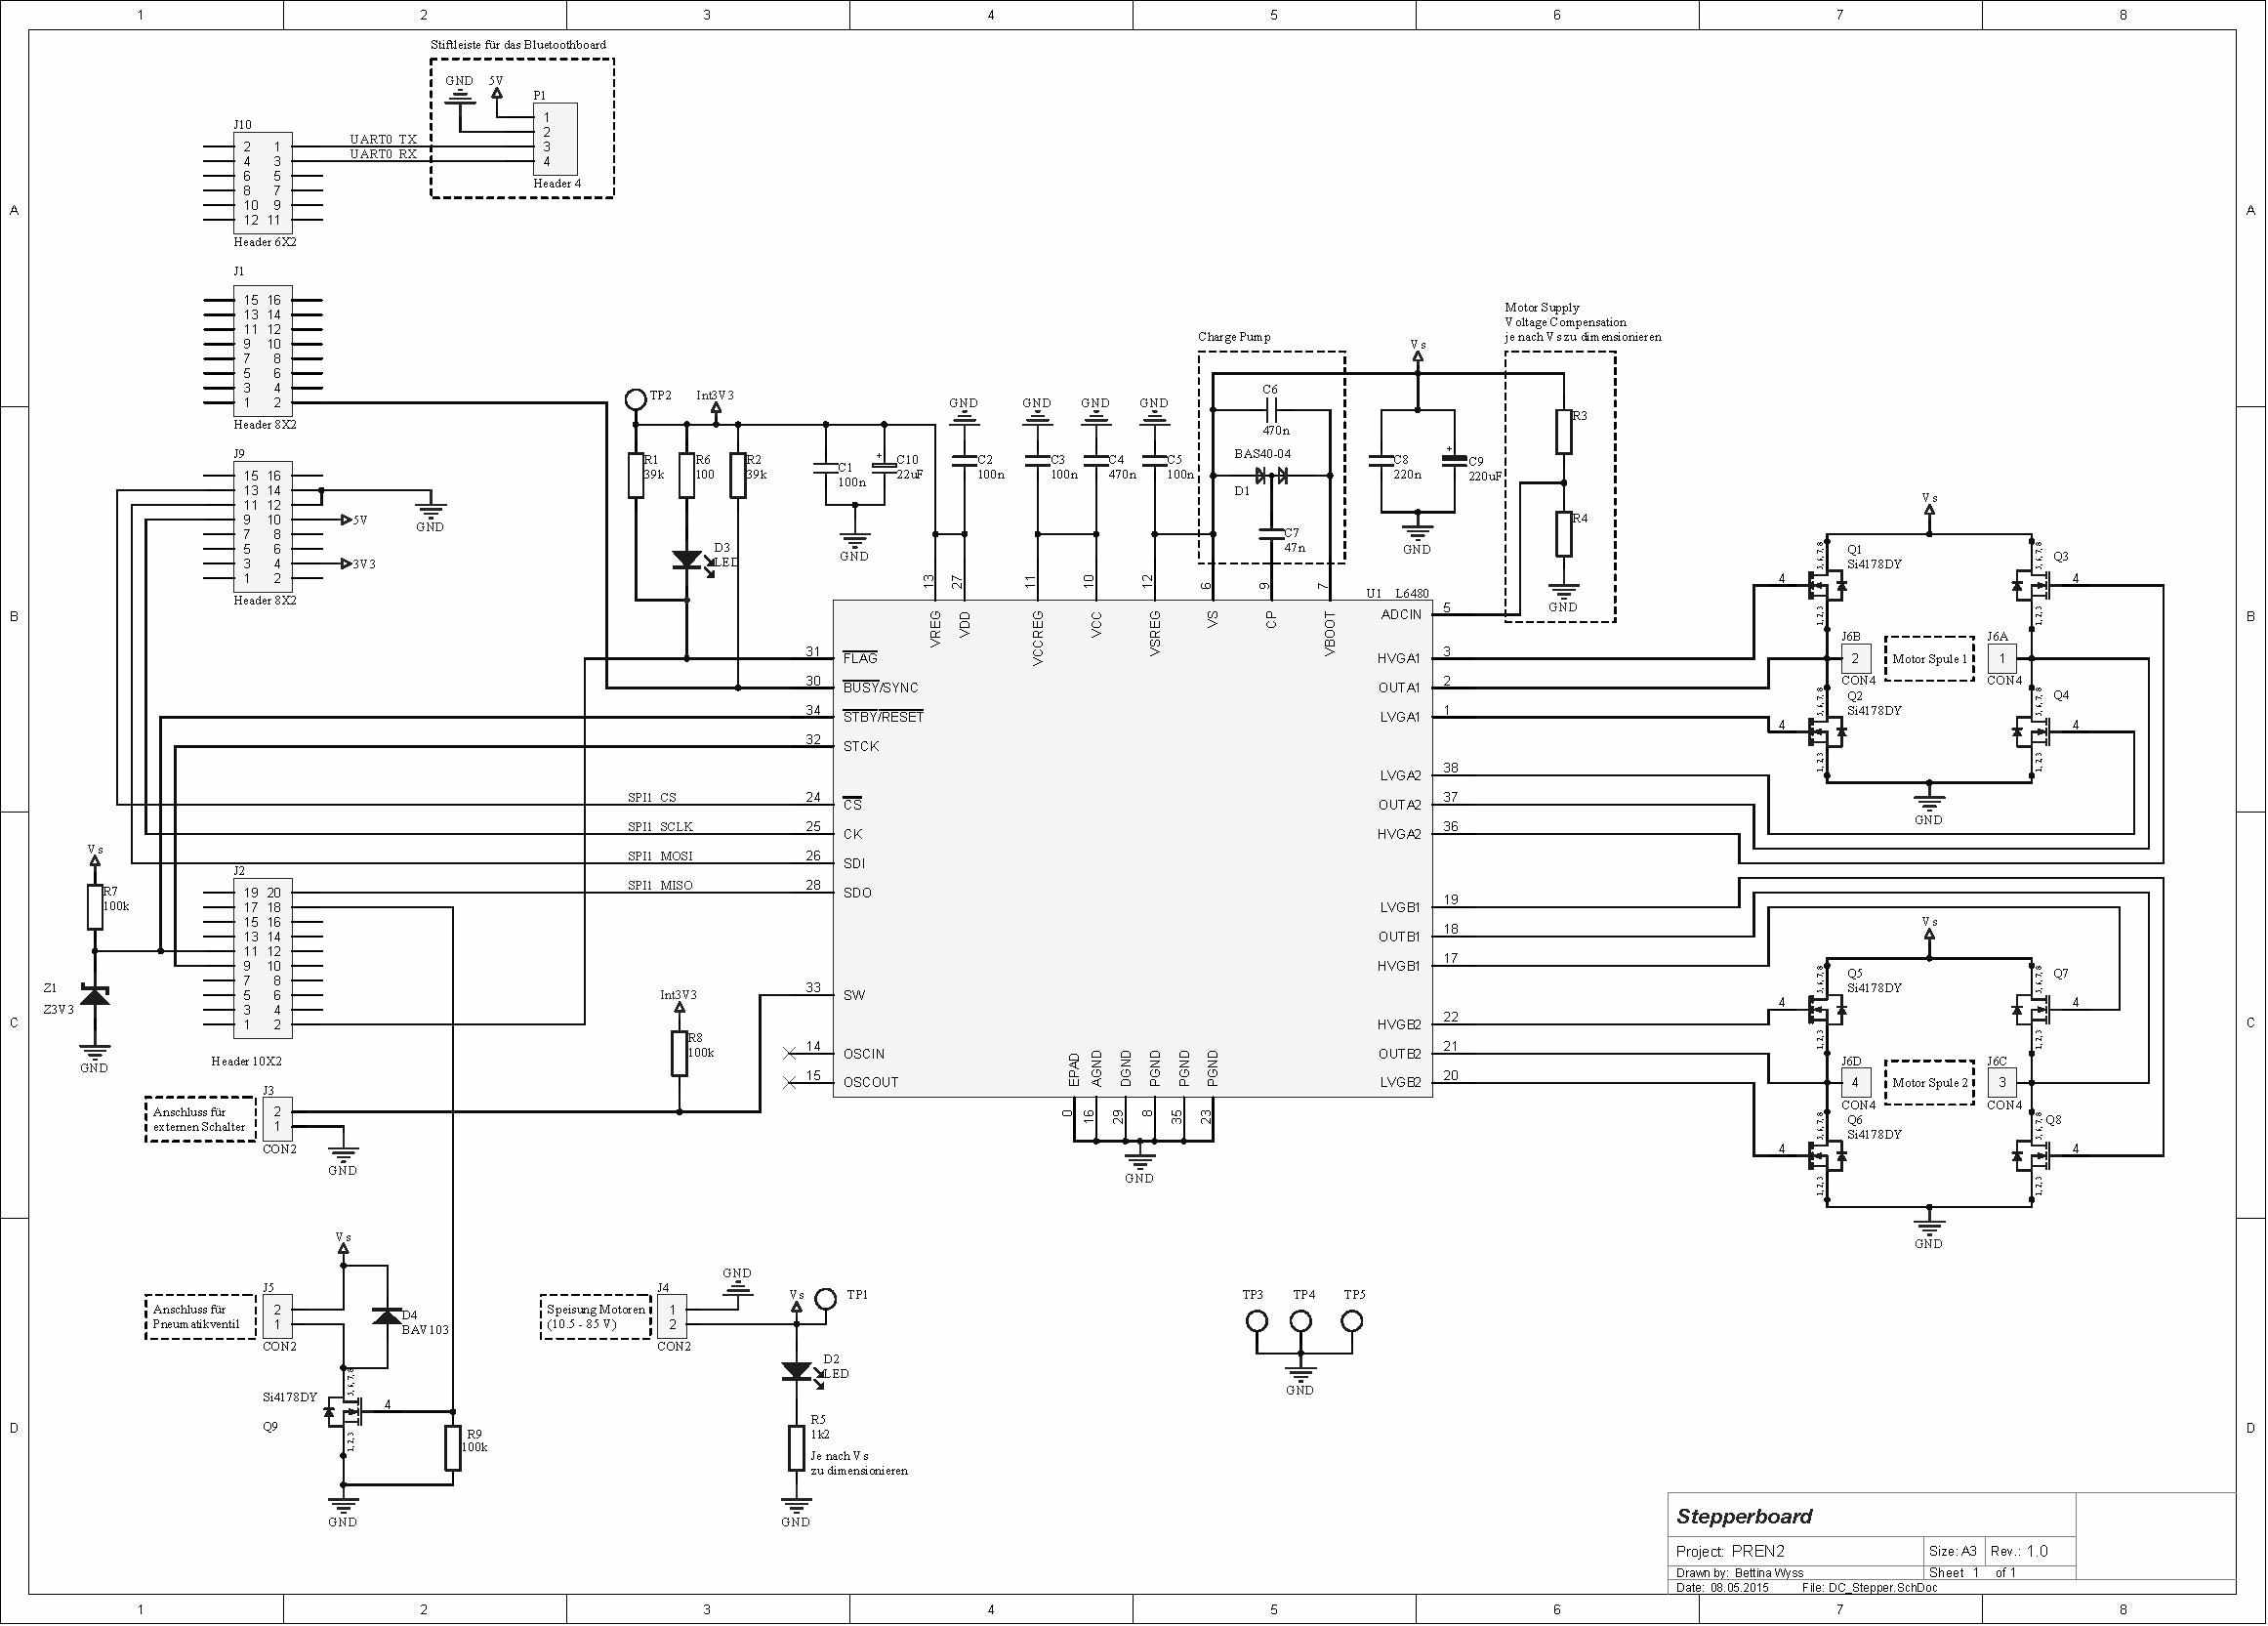
\includepdf[page=1 , offset=0cm -3cm, angle = 90, width=\textwidth,picturecommand={\centering},pagecommand=\subsection*{Schema}\label{Schema}]{\EtPath/Bilder/Stepperboard_Schematic.pdf}
    \newpage
    \subsection*{Bestückungsdokumente}
    \begin{figure}[h!]
        \centering
        \begin{minipage}[hbt]{6cm}
            \centering
            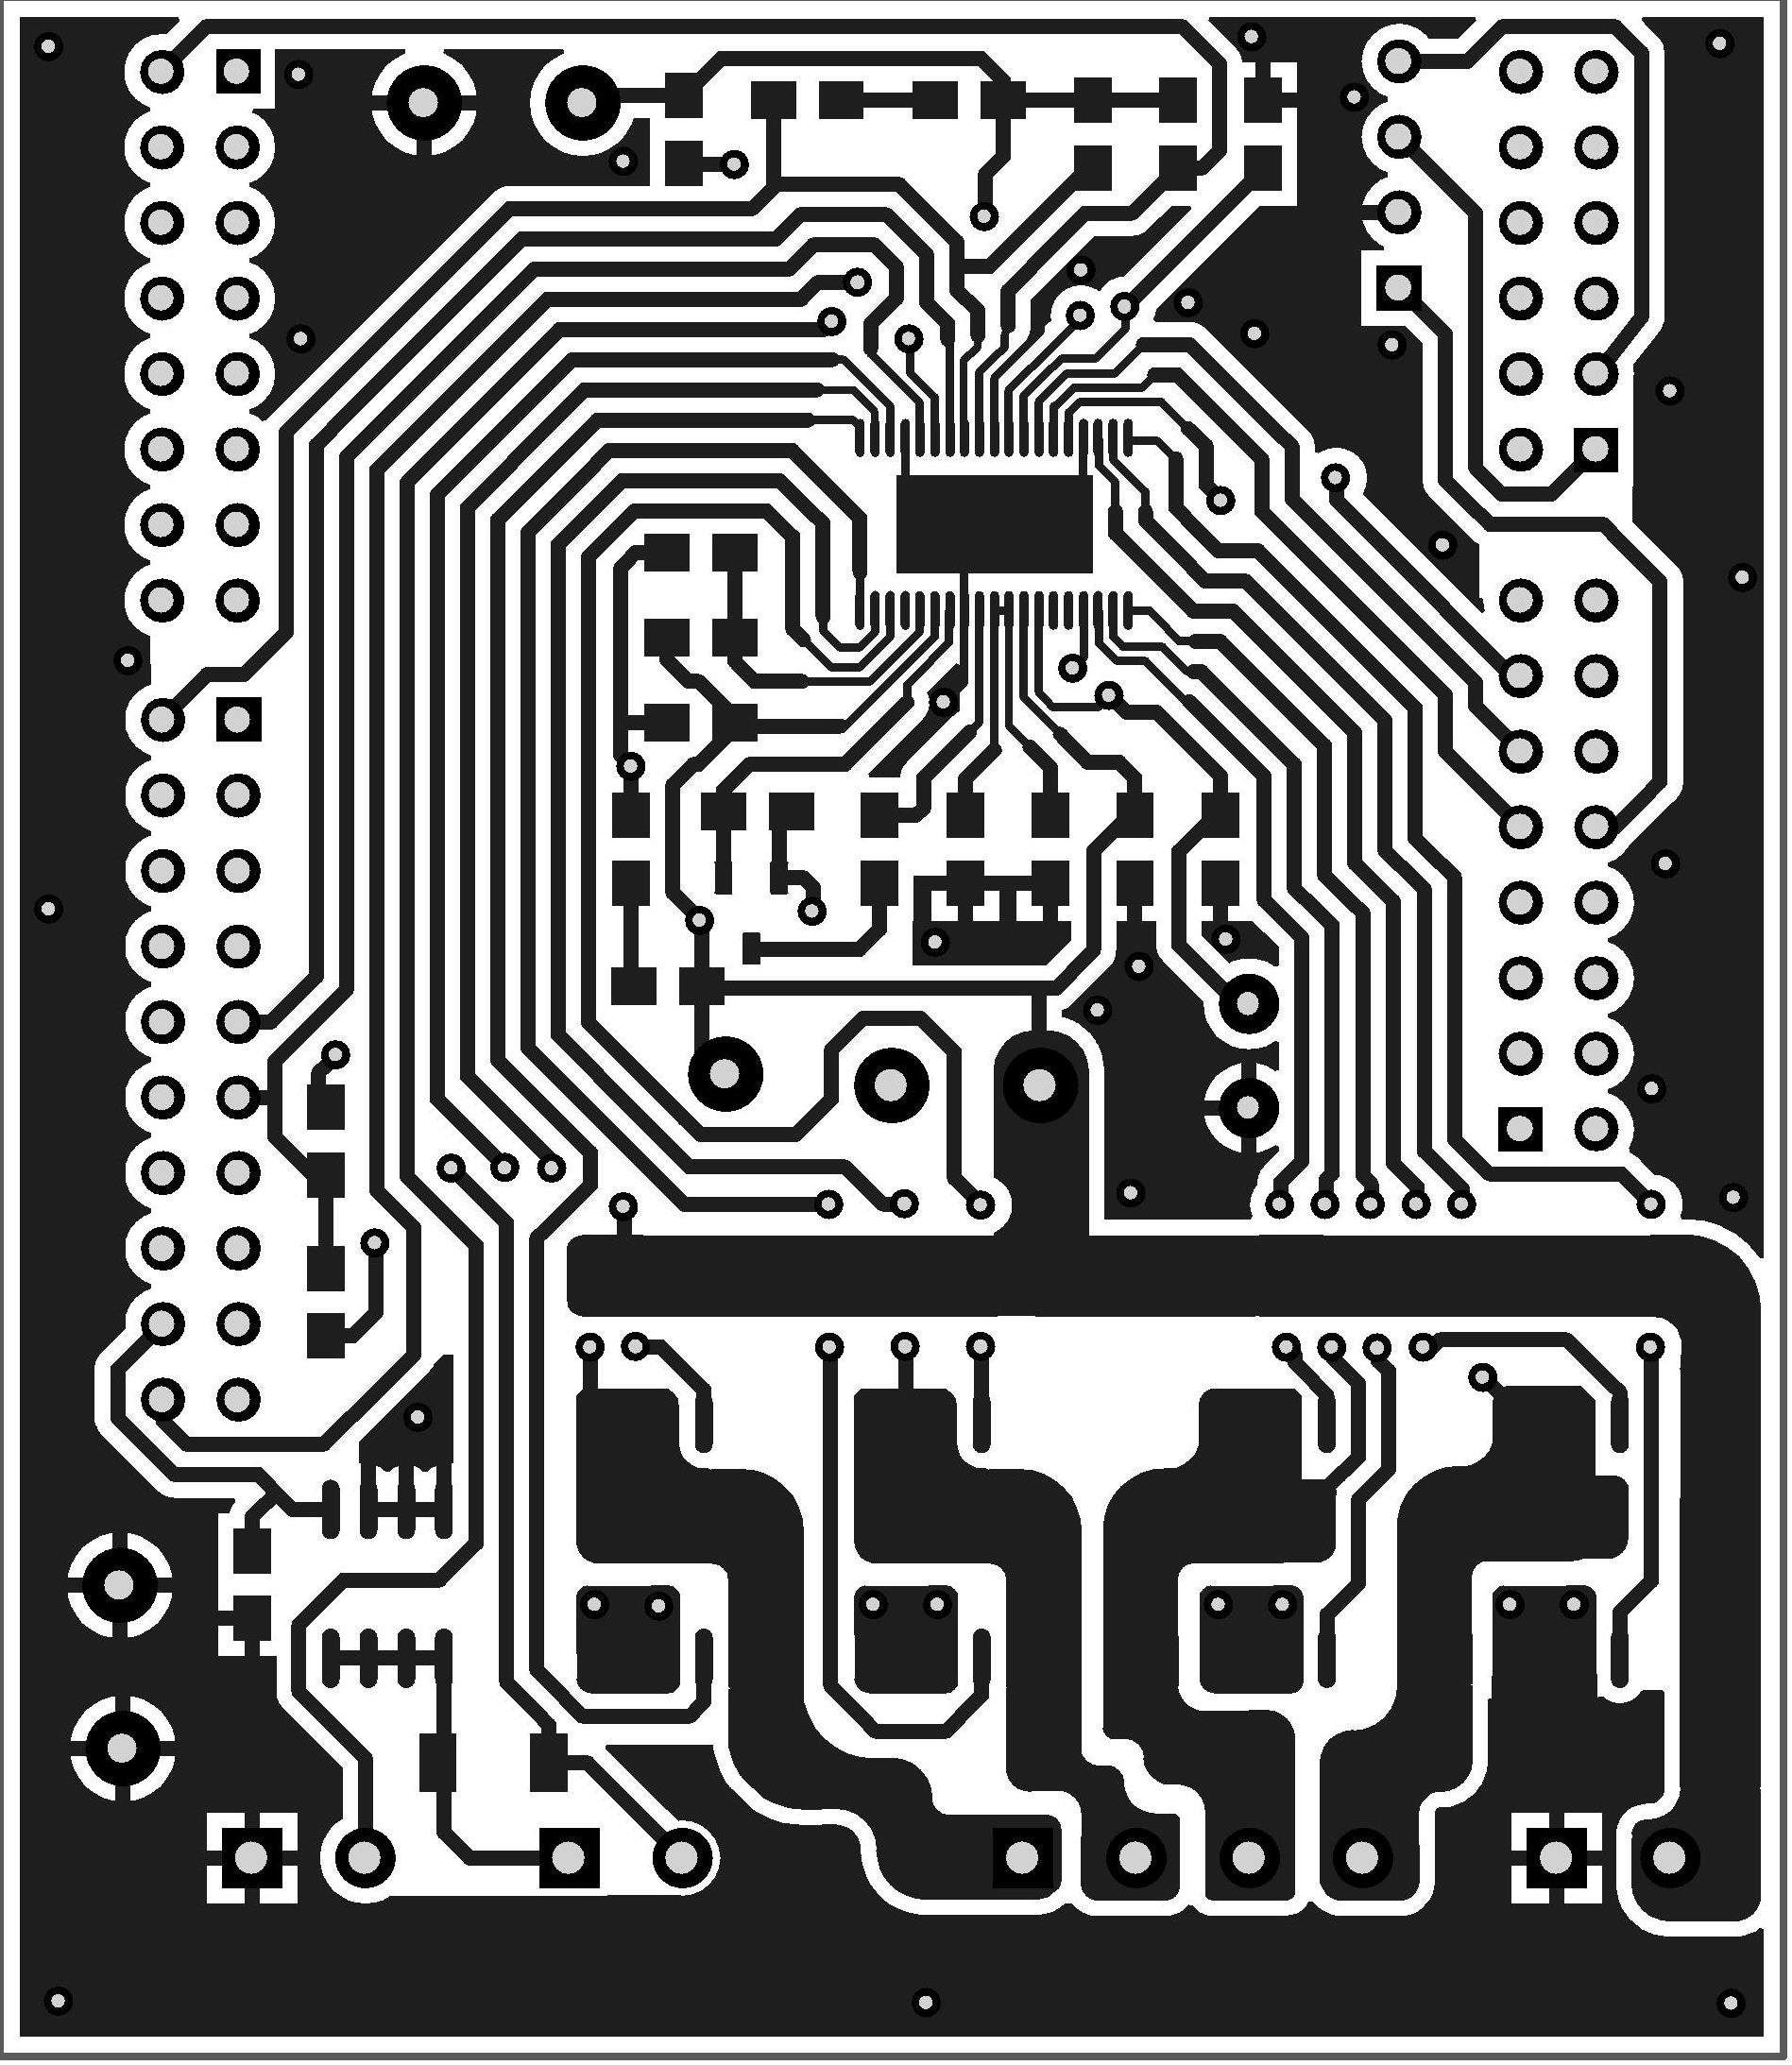
\includegraphics[width=6cm]{\EtPath/Bilder/DC_Stepper0.jpg}
            \caption{Top Layer}
            \label{fig:Top Layer}
        \end{minipage}
        \hspace{1.5cm}
        \begin{minipage}[hbt]{6cm}
            \centering
            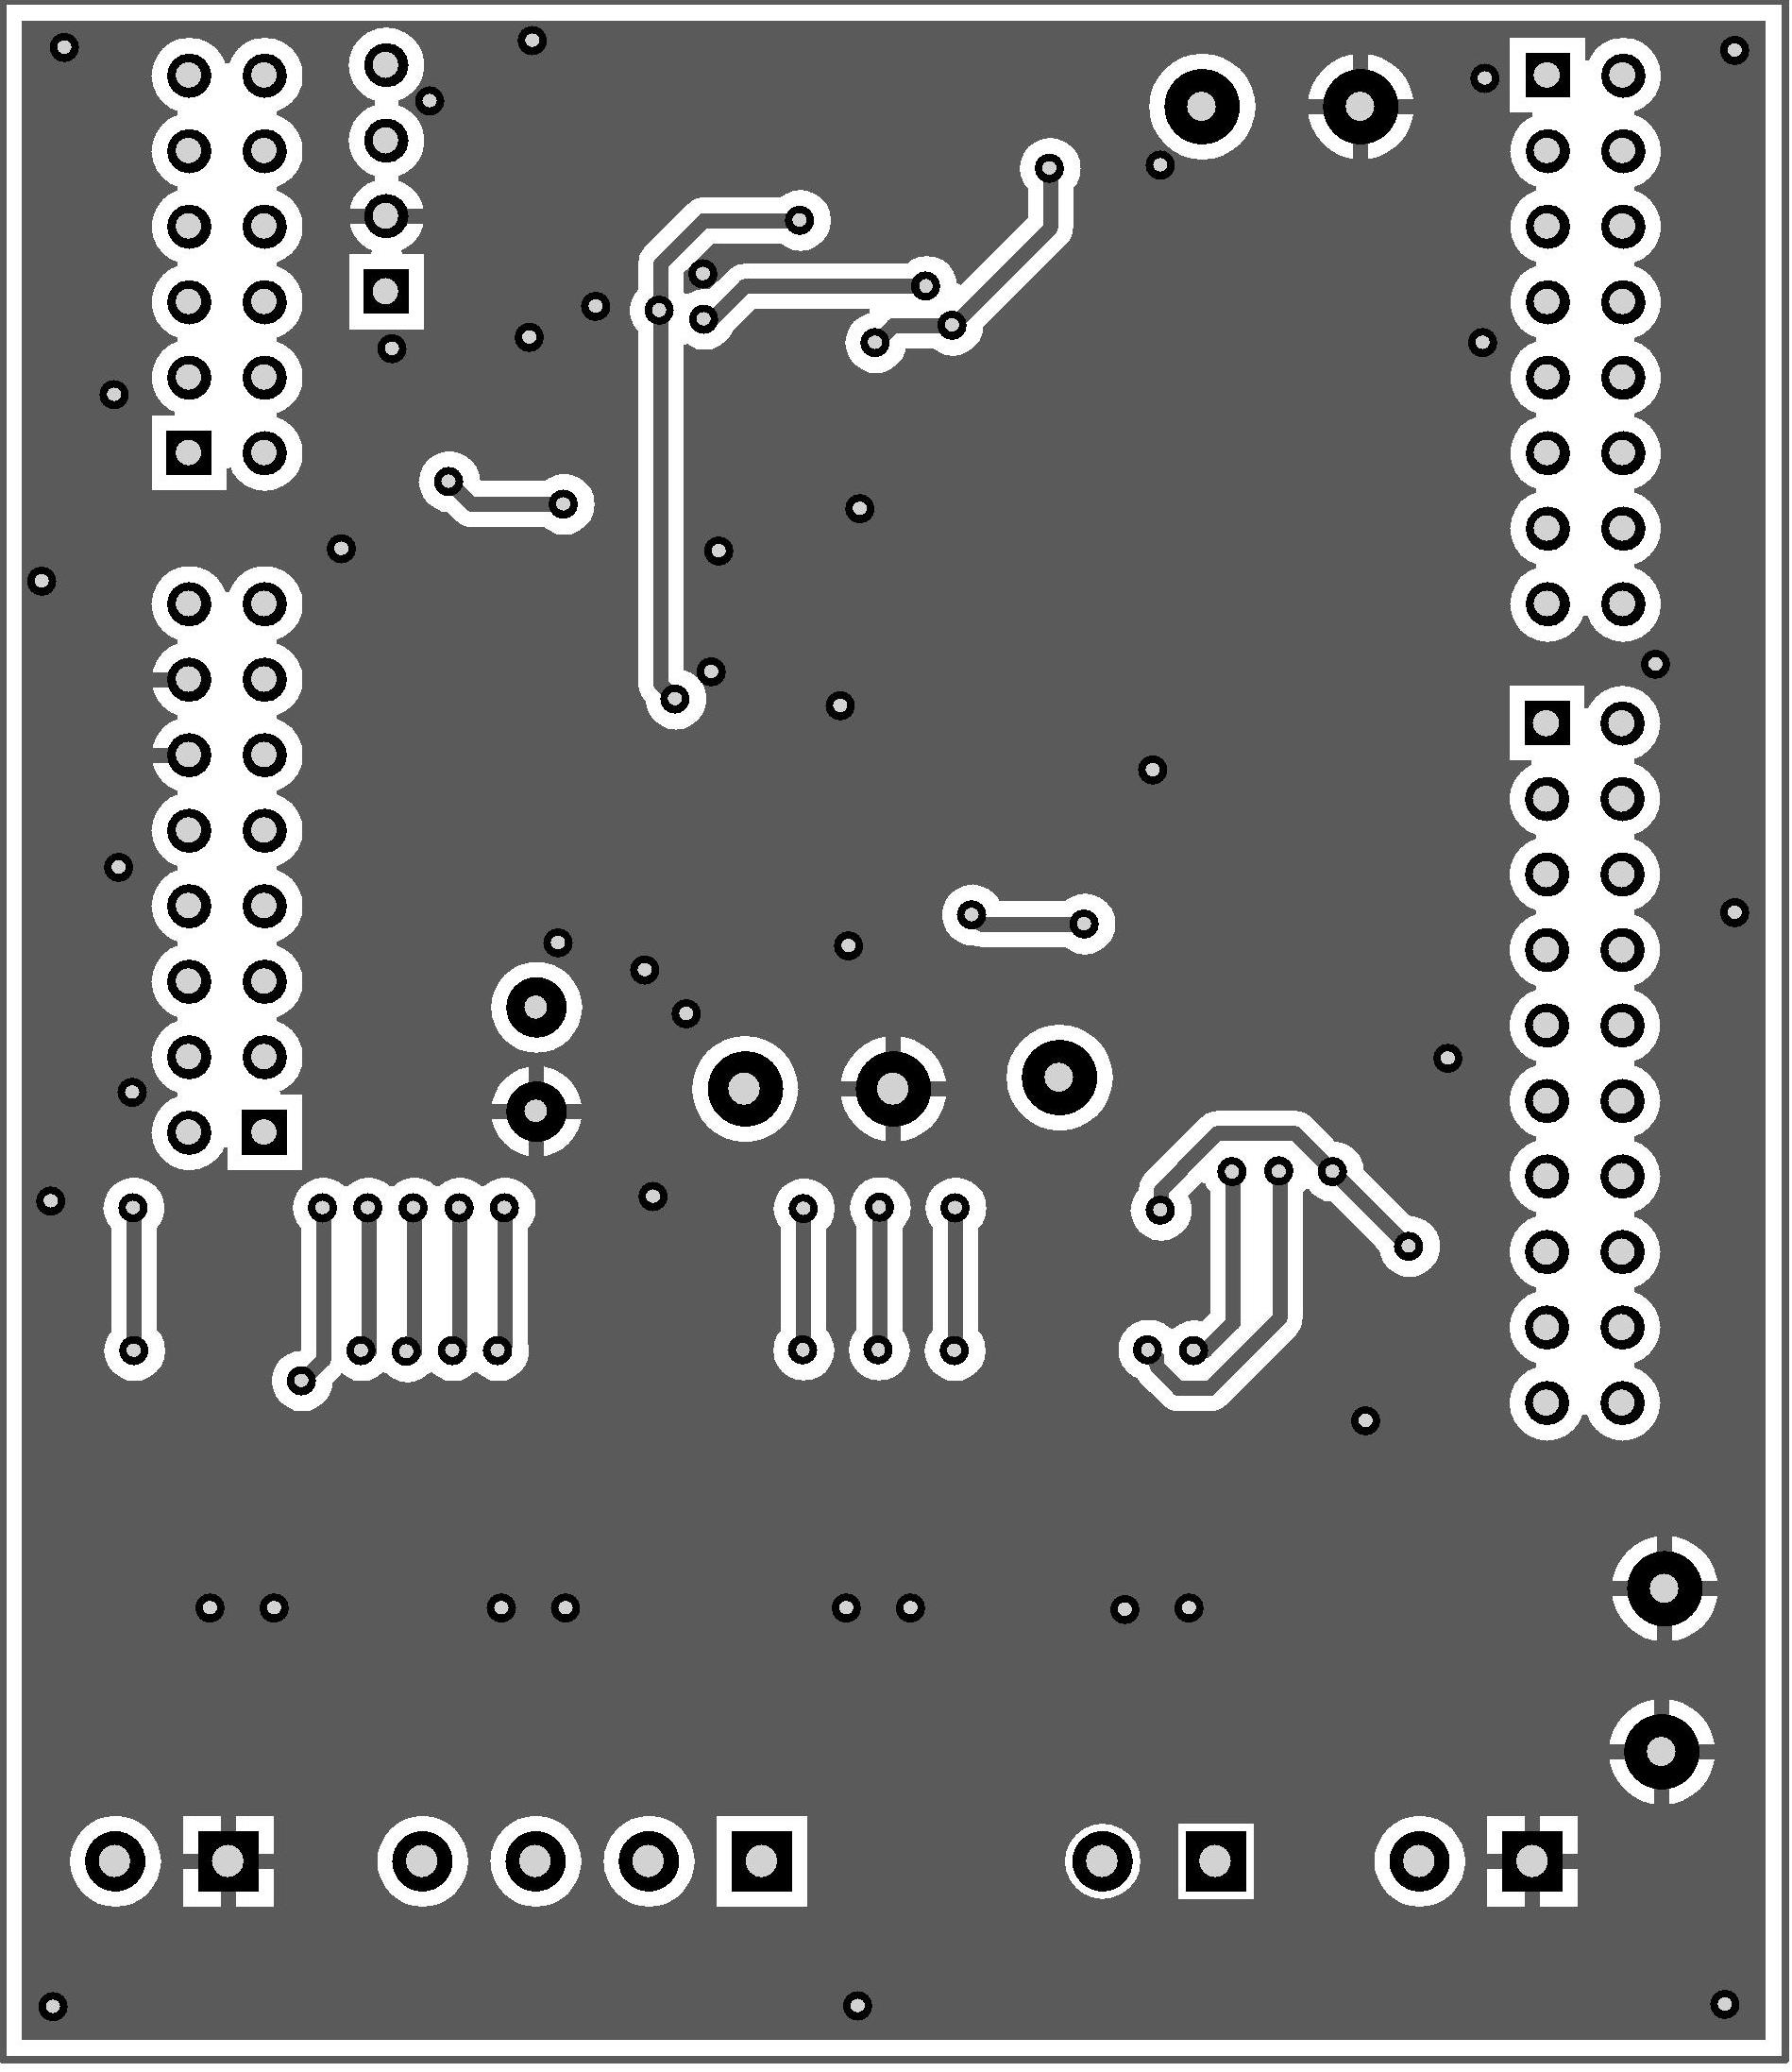
\includegraphics[width=6cm]{\EtPath/Bilder/DC_Stepper1.jpg}
            \caption{Bottom Layer}
            \label{fig:Bottom Layer}
        \end{minipage}
        \\[4ex]
        \begin{minipage}[hbt]{6cm}
            \centering
            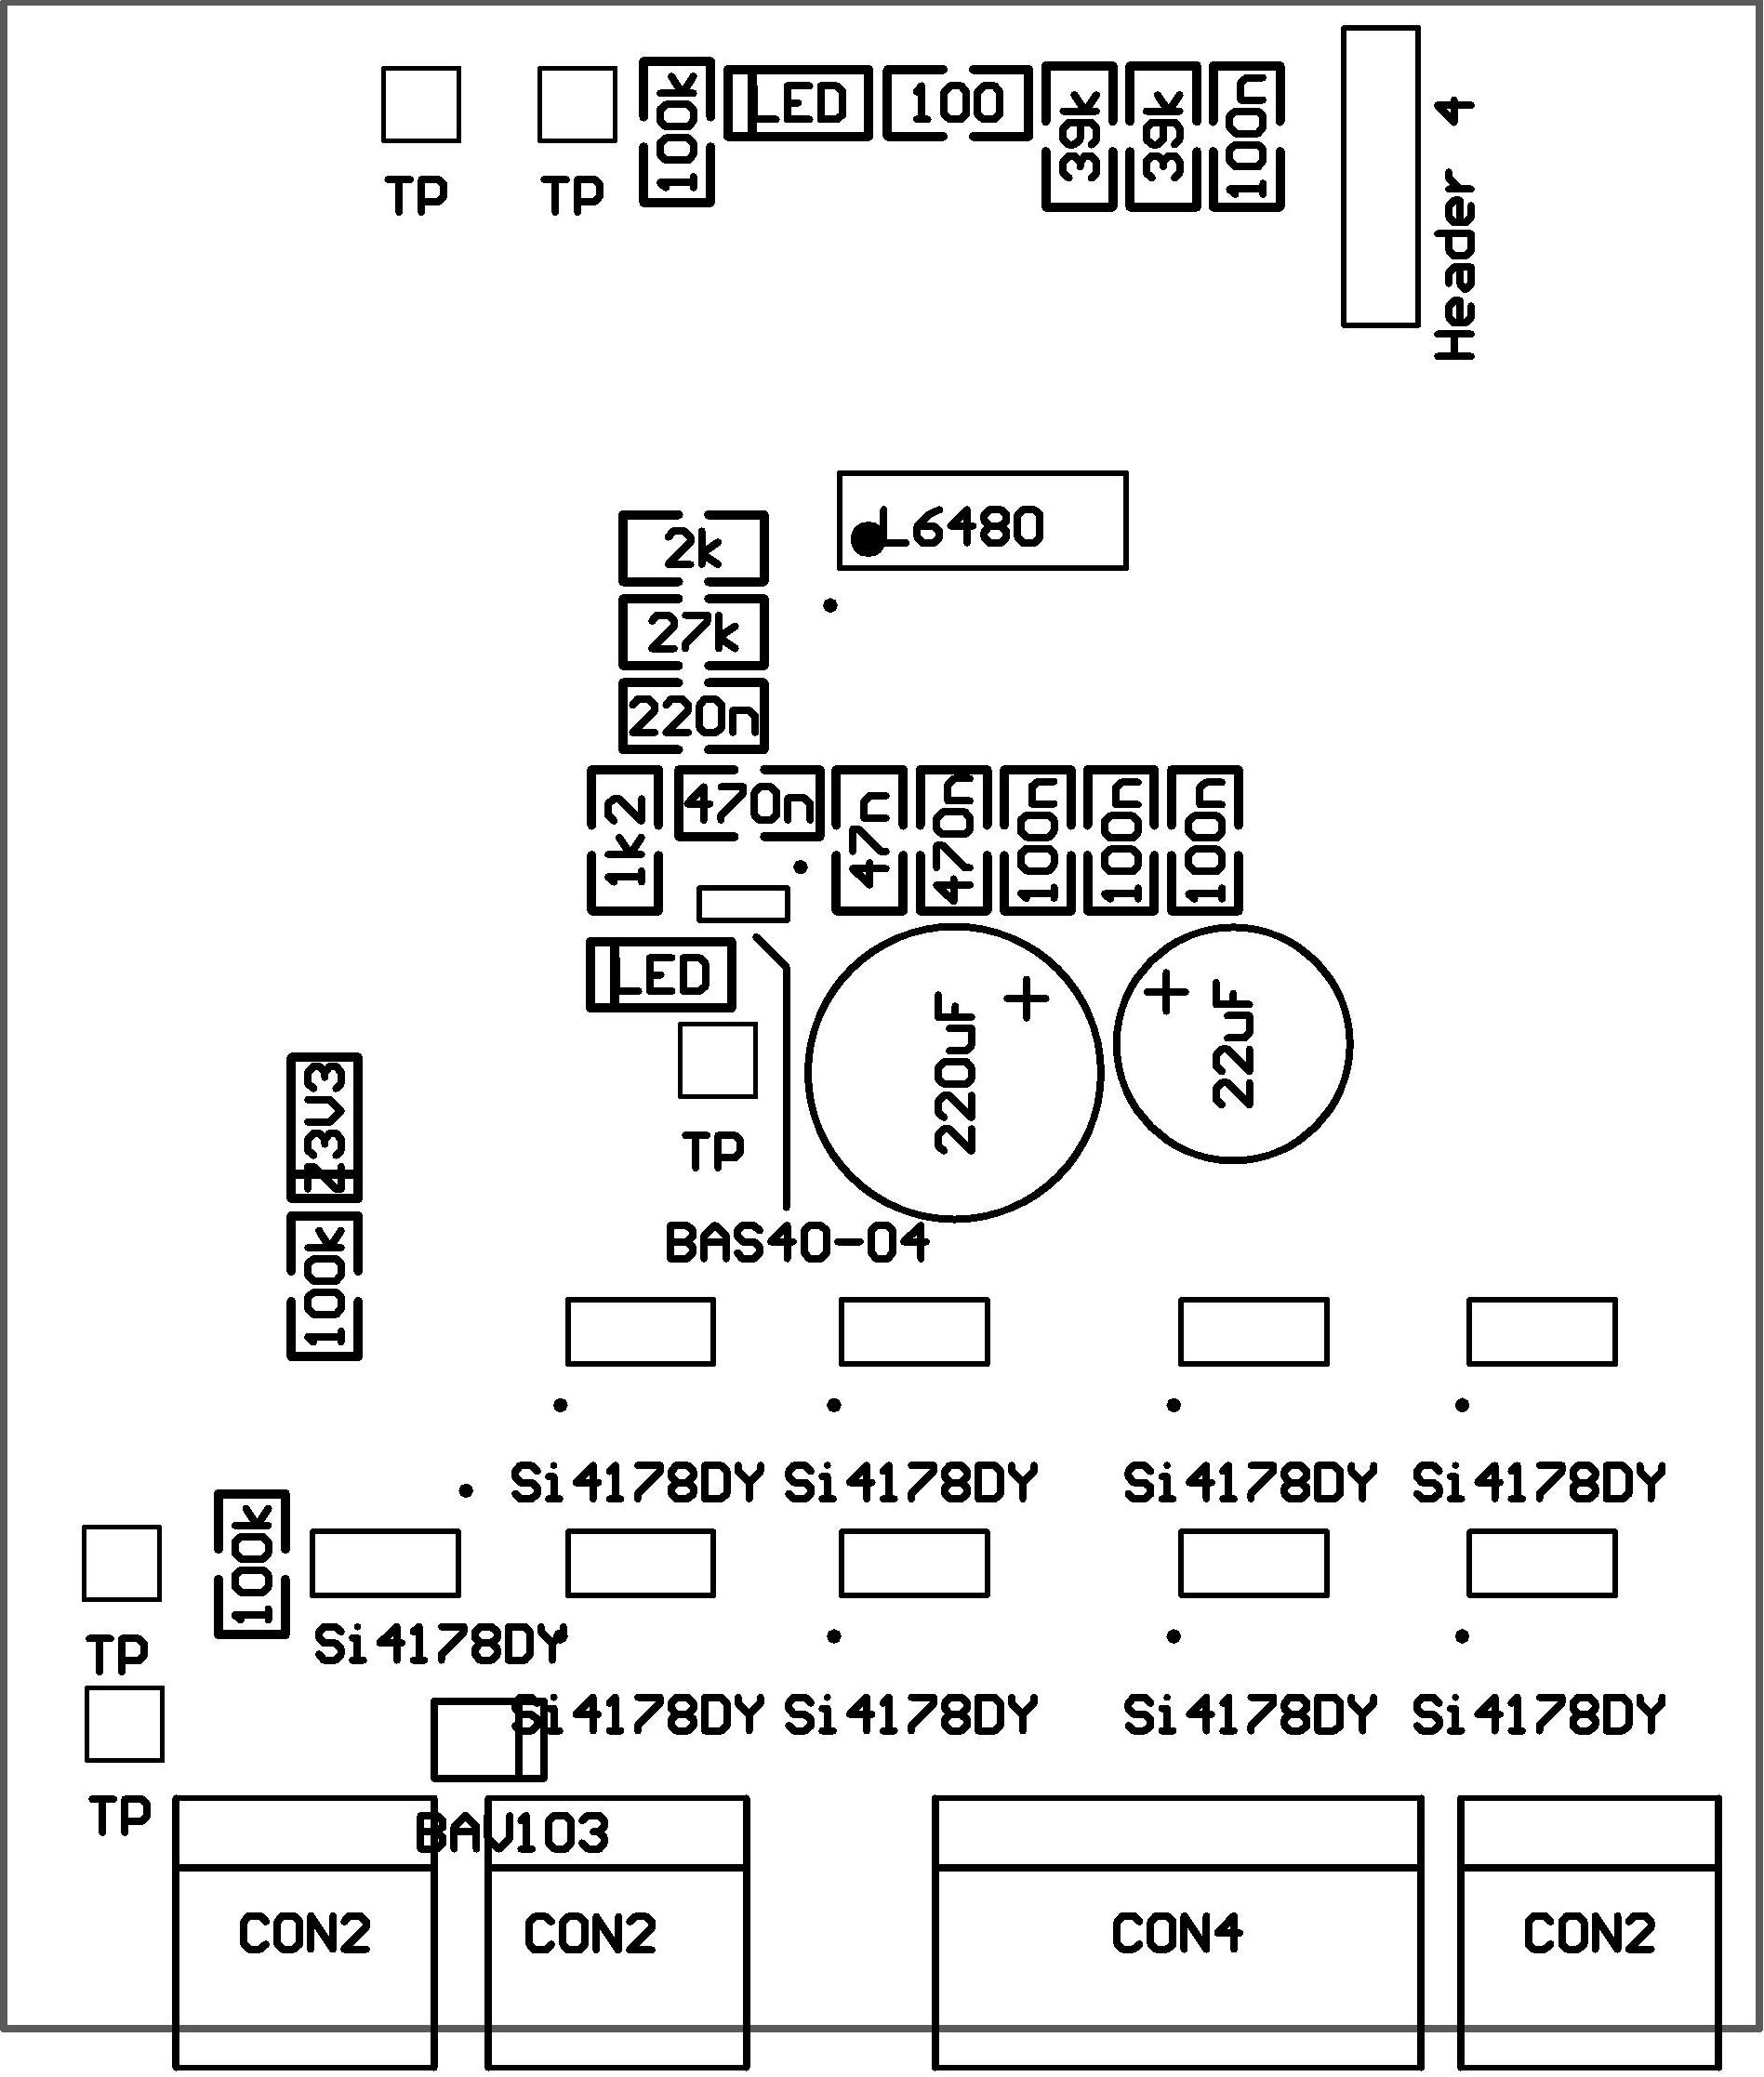
\includegraphics[width=6cm]{\EtPath/Bilder/DC_Stepper2.jpg}
            \caption{Werte}
            \label{fig:Werte}
        \end{minipage}
        \hspace{1.5cm}
        \begin{minipage}[hbt]{6cm}
            \centering
            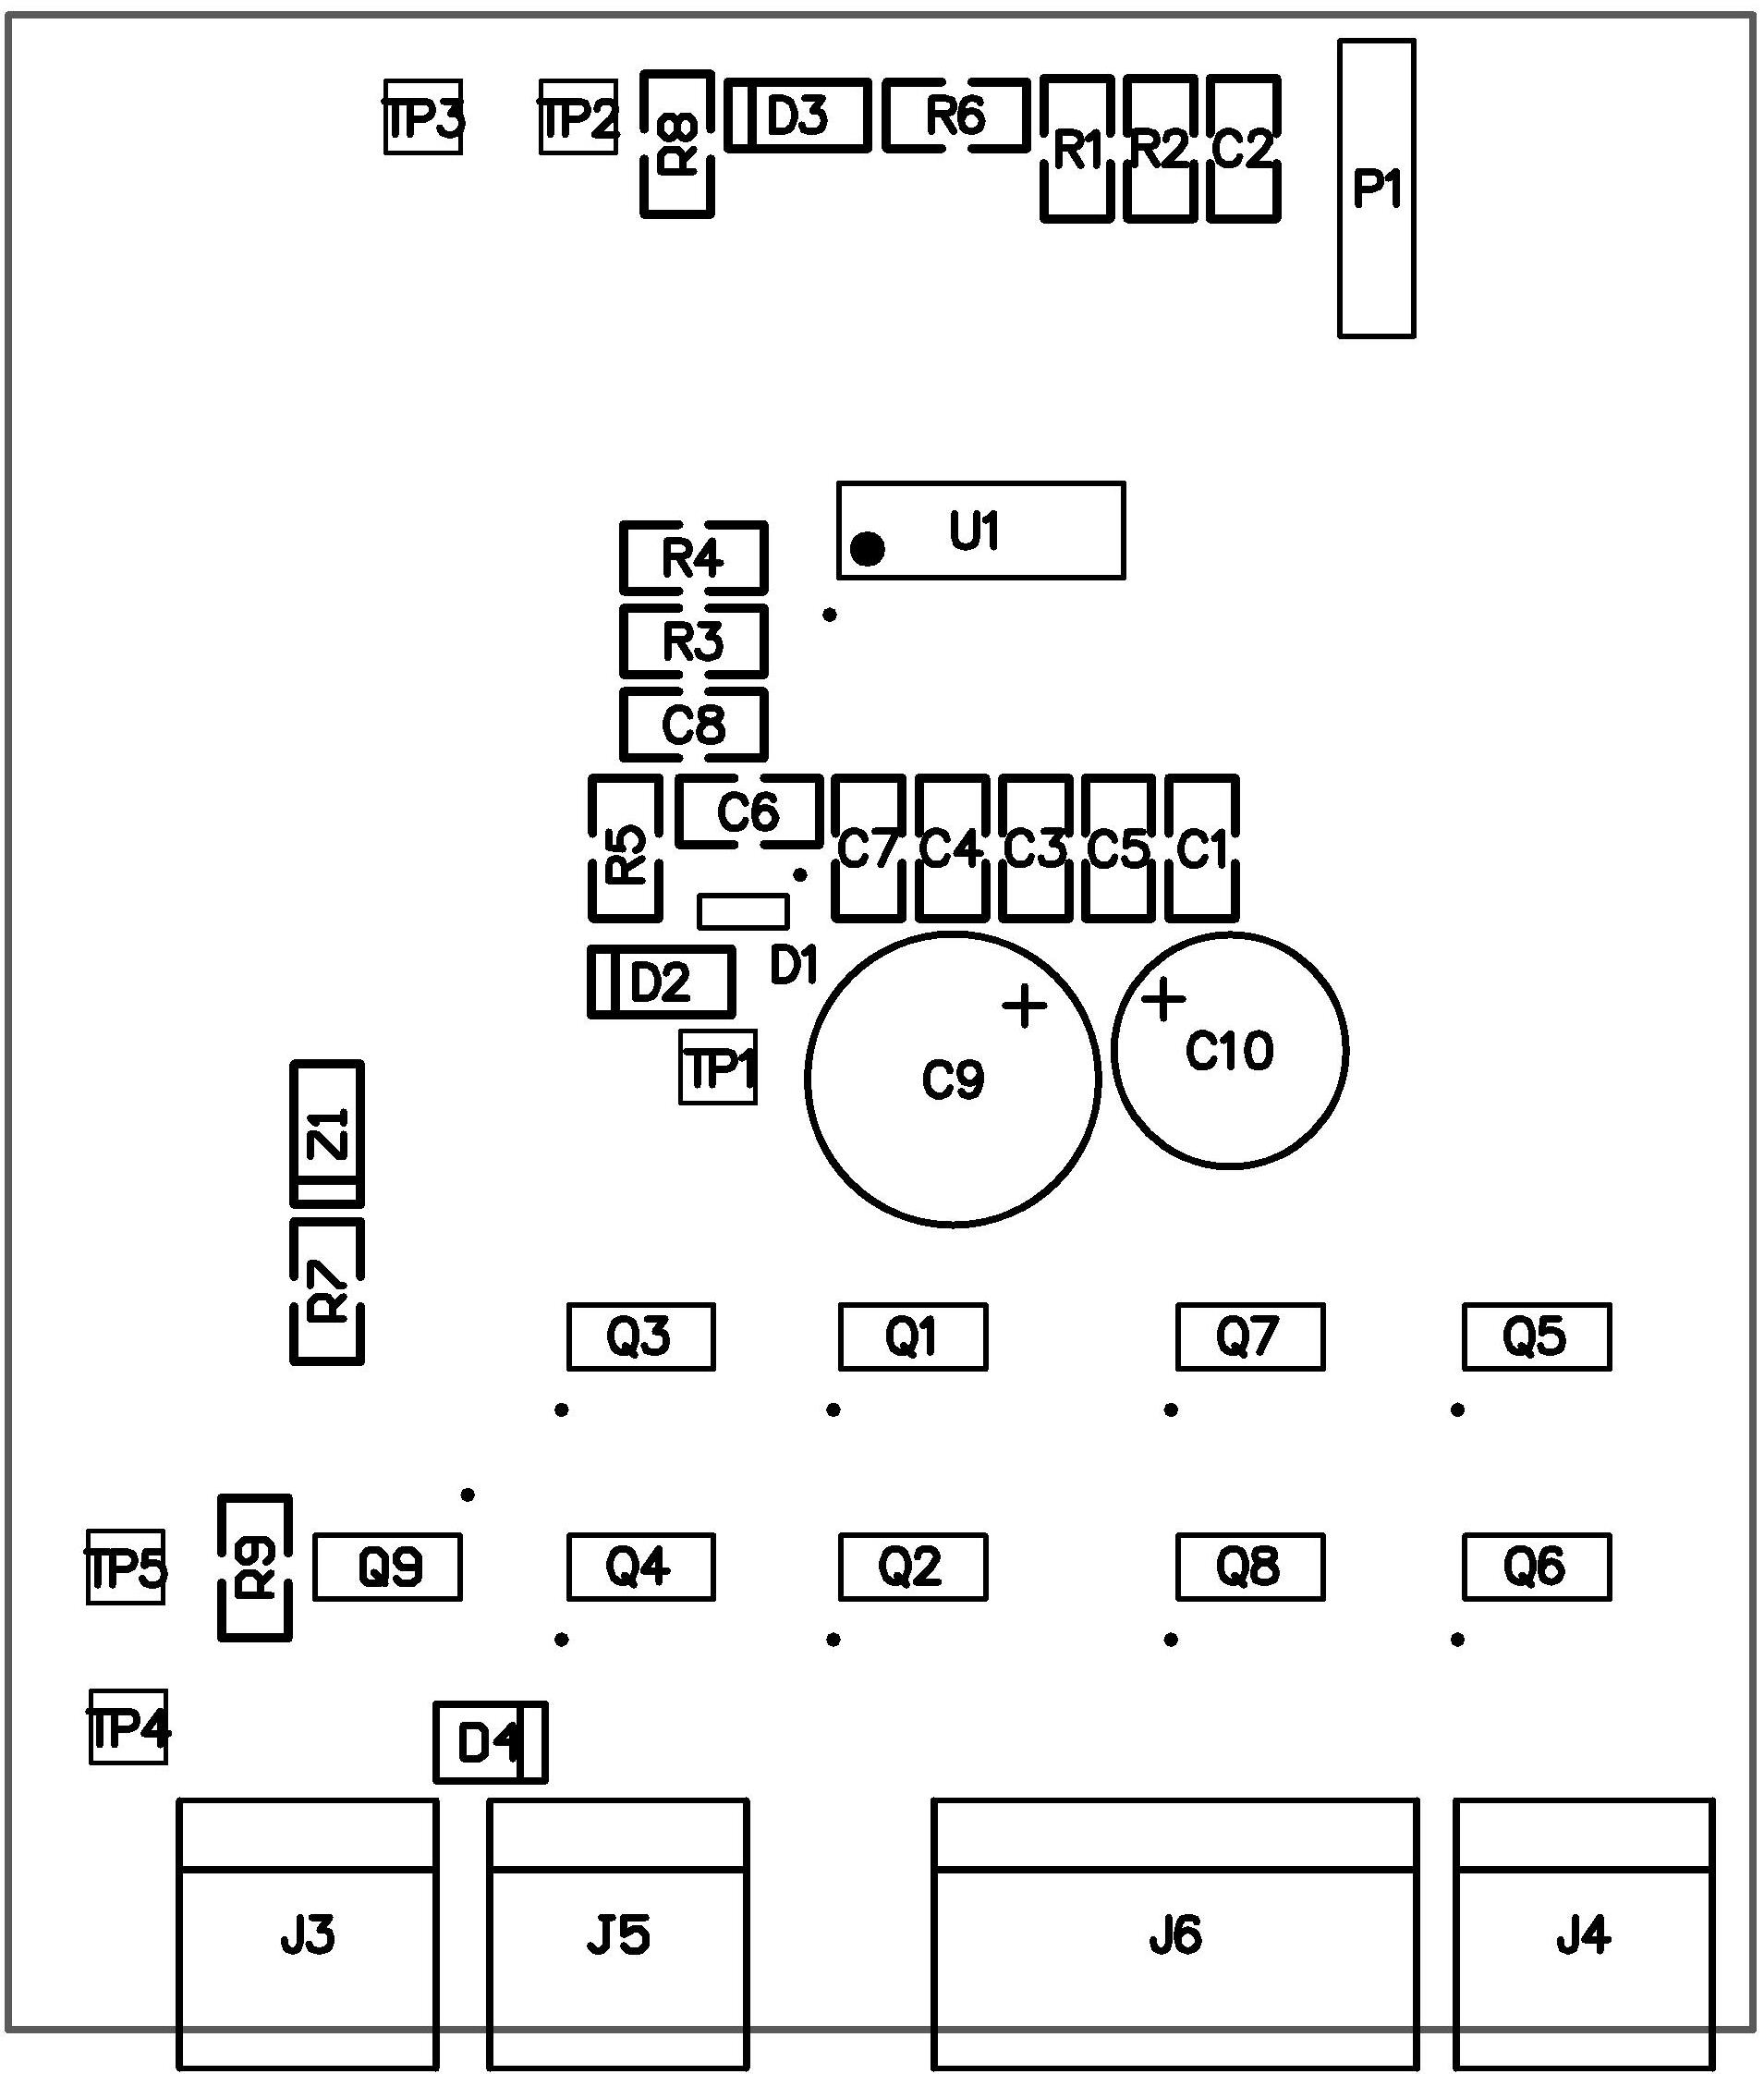
\includegraphics[width=6cm]{\EtPath/Bilder/DC_Stepper3.jpg}
            \caption{Bezeichnungen}
            \label{fig:Bezeichnungen}
        \end{minipage}
    \end{figure}
    % -----------------------------------------------------------------------------------
    \ifSTANDALONE
    \subsection{Print Design} \label{sec:PrintDesign}   
    \fi
    \ifEMBED
    \subsubsection{Print Design} \label{sec:PrintDesigna}
    \fi
    % TODO Betty, Korrektur durch Clirim        
    Der Adapterprint soll auf das Freedom-Board aufgesteckt werden und 
    möglichst klein sein. Der Print hat eine Grösse von 60mm x 70mm. Darauf 
    befinden sich die Anschlüsse für die Speisung, für den Motor, für weitere 
    Motoren und für einen End- oder Notschalter. Dazu werden stabile 
    Leiterplattenanschlüsse gewählt, welche auch die hohen Phasenströme des 
    Motors aushalten und zudem eine genug hohe Spannungsfestigkeit besitzen, 
    da die Motorenspannung bis 85V gewählt werden kann. Die eingesetzten 
    Leiterplattenanschlüsse sind für eine Spannung bis 300V und einem Strom 
    bis 8A geeignet. Dies ist ausreichend für diese Anwendung. Alle Bauteile 
    sind SMD, ausser den Leiterplattenanschlüssen und den Kondensatoren.
    \newpage
    Grundsätzlich werden folgende Regeln beim Design eingehalten: 
    \begin{itemize}
        \item Leiterbahnbreite 20mil
        \item Abstände zwischen Leiterbahnen und Polygonen 20mil
        \item keine rechten Winkel
        \item möglichst wenig Auskreuzungen auf dem Bottomlayer
        \item genügend grosse Pads 
        \item Verbindungen möglichst kurz halten
    \end{itemize}
    Da die Pins des L6480 näher als 20mil zueinander sind, können dort die 
    Regel für die Leiterbahnbreite und für den Abstand nicht eingehalten 
    werden. Deshalb werden für dieses Bauteil eigene Regeln definiert. Die 
    Leiterbahnen sind um den L6480 nur 8mil breit, werden jedoch sofort auf 
    20mil verdickt. Die Motorenphasen werden nicht mit Leiterbahnen an die 
    Anschlüsse geführt, sondern mit breiten Polygonen verbunden. Die 
    Auskreuzungen auf dem Bottomlayer werden vermieden, da einerseits 
    der erste Prototyp ohne Durchkontaktierung hergestellt wird, andererseits 
    da die GND-Fläche auf dem Bottomlayer möglichst nicht "verschnitten" 
    werden soll, um so EMV-Störungen abzuschirmen.
    Nach dem Layouten des ersten Prototypes folgt das Bestellen der Bauteile, 
    welche nicht im Elektroniklabor vorhanden sind. Die Stückliste ist in der 
    \autoref{Stückliste} zu finden. Der erste Prototyp wird von Hand 
    durchkontaktiert. Nach dem Bestücken mit der halbautomatischen 
    Bestückungsmaschine und dem Löten im Ofen wird der Prototyp in Betrieb 
    genommen. Die Inbetriebnahme zeigt, dass einige wenige Änderungen im 
    Layout nötig sind. Diese werden in einer überarbeiteten Version des 
    Adapterprints berücksichtigt. Der zweite Print wird maschinell 
    durchkontaktiert. Die Dokumente zur ersten Version sind im Anhang zu 
    finden. Die Bestückungsdokumente sind auf Seite \pageref{fig:Bottom Layer} 
    abgebildet.
    \begin{figure}[h]
        \centering
        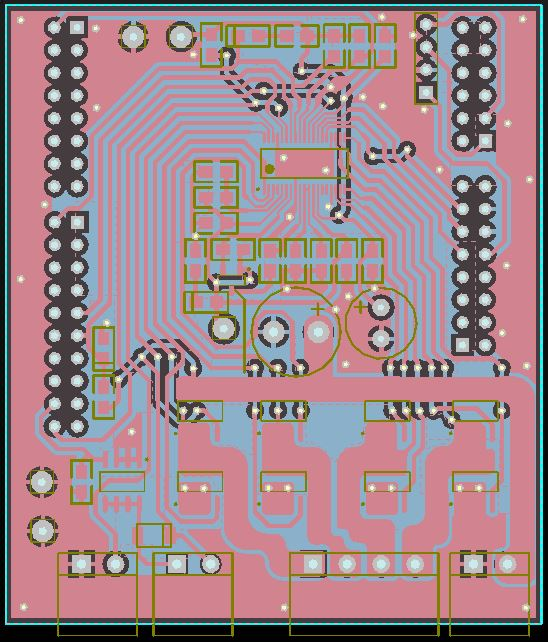
\includegraphics[width=5cm]{\EtPath/Bilder/printdesign.JPG}
        \caption{Printdesign mit Altium Designer}
        \label{fig:printdesign}
    \end{figure}
    \begin{table}
        \begin{zebralongtable}{p{2.5cm} p{3cm} p{2cm} p{4cm} p{1cm}} 
            \rowcolor{gray}
            \textbf{Bauteil}    & \textbf{Bezeichnung}  & \textbf{Lieferant} & \textbf{Bestellnummer}   &\textbf{Anz}\\
            Motor Contoller     & L6480H                & Mouser             & 511-L6480H               & 1\\   
            Shottkydiode        & BAS40-04-G            & Mouser             & 78-BAS40-04-E3-08        & 1\\ 
            Zenerdiode          & BZX585-B3V3           & Mouser             & 771-BZX585-B3V3          & 1\\ 
            Freilaufdiode       & BAV103                & Mouser             & 512-BAV103               & 1\\ 
            FET                 & Si4178DY              & PTA16              & 781-SI4178DY-TI-GE3      & 9\\ 
            LED                 & LSQ976                & Mouser             & 720-LSQ976-NR-1          & 2\\ 
        \end{zebralongtable}
        \caption{Stückliste (Bauteile nicht an Lager)} 
        \label{Stückliste}
    \end{table}  
    \newpage
    % -----------------------------------------------------------------------------------
    \ifSTANDALONE
    \subsection{Software}   \label{ch:Software} 
    \fi
    \ifEMBED
    \subsubsection{Software} \label{ch:Software}
    \fi
    Für die einfache Einbindung des Schrittmotortreibers in die Software der 
    jeweiligen Teams wird eine Bibliothek erstellt. Diese besteht aus den 
    Dateien \verb?l6480.c? und \verb?l6480.h?, welche in eigene Software 
    eingebunden werden kann. 
    \begin{lstlisting}[caption={Einbinden der Bibliothek}]
#include l6480.h
    \end{lstlisting}
    Diese Bibliothek bietet Funktionen um alle Register des 
    Schrittmotortreibers zu beschreiben und zu lesen. Ausserdem ist jeder 
    Befehl des Treibers implementiert. Die Bibliothek ist mit Doxygen 
    dokumentiert. In der entsprechenden Dokumentation ist die Schnittstelle 
    der Bibliothek beschrieben. 
    Damit die Bibliothek mit dem Schrittmotortreiber kommunizieren kann, muss 
    eine SPI Schnittstelle zur breeitgestellt werden. Dazu sind die Funktionen 
    \verb?spi_write(uint8_t *data)? und \verb?spi_read(uint8_t *data)? so zu 
    ergänzen, dass sie jeweils ein Byte über SPI senden respektive empfangen.  
    Über die Konstante \verb?PL_FRDM? ist die SPI Schnittstelle auf einem 
    FRDM-KL25Z von Freescale einschaltbar. Die SPI Komponente heisst dabei 
    Stepperspi. Alle notwendigen Komponenten sind in \autoref{tab:comp_frdm} 
    aufgeführt. 
    \begin{lstlisting}[caption={Definition der Plattform für das FRDM-KL25Z}]
#define PL_FRDM
    \end{lstlisting}
    \begin{table}[h!]
        \centering
        \begin{zebratabular}{p{0.11\textwidth}p{0.14\textwidth}p{0.5\textwidth}}
            \rowcolor{gray}
            Name        & Komponente    & Beschreibung \\
            Stepperspi  & SynchroMaster & SPI \\
            WAIT1       & Wait          & Delays \\
            STP\_BSY    & ExtInt        & Interrupt für das Signal Busy \\
        \end{zebratabular}
        \caption{Komponenten bei Verwendung auf einem FRDM-KL25Z}
        \label{tab:comp_frdm}
    \end{table}
    Zudem kann mit der Konstante \verb?PL_HAS_SHELL?  die Unterstützung einer 
    Shell-Komponente aktiviert werden. Die für die Shell zusätzlich 
    notwendigen Komponenten sind in \autoref{tab:comp_shell} aufgeführt. 
    \begin{lstlisting}[caption={Definition für Shell-Unterstützung}]
#define PL_HAS_SHELL
    \end{lstlisting}
    \begin{table}[h!]
        \centering
        \begin{zebratabular}{p{0.11\textwidth}p{0.14\textwidth}p{0.5\textwidth}}
            \rowcolor{gray}
            Name        & Komponente    & Beschreibung \\
            CLS1        & Shell         & Shell \\
            UTIL1       & Utility       & Funktionen für die Verarbeitung von Strings \\
            Shell       & -             & Funktionen für das Senden von Strings über die Schell \\
        \end{zebratabular}
        \caption{Komponenten bei Verwendung der Shell}
        \label{tab:comp_shell}
    \end{table}

    \clearpage
    \ifSTANDALONE
    \subsubsection{Test auf Computer}   \label{sec:Software_test} 
    \fi
    \ifEMBED
    \paragraph{Test} auf Computer \label{sec:Software_test}
    \fi
    Wird die Konstante \verb?PL_FRDM?  nicht gesetzt, kann die Bibliothek auf 
    einem Computer kompiliert und getestet werden. Das ermöglicht das Testen 
    der Bibliothek ohne Hardware. Die Daten werden dabei nicht über SPI 
    geschickt, sondern auf die Standardausgabe ausgegeben. 
    \begin{lstlisting}[caption={Beispielprogramm für den Test der Bibliothek auf dem Computer}, label={lis:test_source}]
#include "stdio.h"
#include "drv/l6480.h"

int main(void) {
    l6480_init();
    printf("hardhiz\n");
    l6480_cmd_hardhiz();
    printf("run 1 2\n");
    l6480_cmd_run(1, 2);
    return 0;
}
    \end{lstlisting}
    \begin{lstlisting}[caption={Ausgabe vom Testprogramm in \autoref{lis:test_source}}]
hardhiz
write: 0xA8
run 1 2
write: 0x51
write: 0x0
write: 0x0
write: 0x2
    \end{lstlisting}






%    Die Software auf dem Freedom-Board dient als Schnittstellensoftware. Sie 
%    nimmt die Befehle der zentralen Recheneinheit über USB/UART an und sendet 
%    diese an den Motor Controller l6480 sowie das Pneumatikventil weiter. Die 
%    Software wurde mit der Entwicklungsumgebung Kinetis Design Studio von 
%    Freescale entwickelt. Diese Umgebung bietet ein Tool, welches Processor 
%    Expert heisst. Dieses erlaubt es, Komponenten wie z.B. einen 
%    Analog-Digital-Wandler in das Projekt zu integrieren. Die Konfiguration 
%    solcher Komponenten kann mit dem Component Inspector vorgenommen werden, 
%    ohne dass einzelne Register des Mikrocontrollers beschrieben werden 
%    müssen. Die Komponenten stammen von der Internetseite 
%    http://steinerberg.com/EmbeddedComponents/ und können dort gratis 
%    gedownloadet werden.
%    \\\\
%    Die Software auf dem Freedom-Board beinhaltet folgende fünf Komponenten 
%    mit ihren Aufgaben: 
%    \begin{itemize}
%        \item FreeRTOS:         Ein Open-Source-Echtbetriebszeitsystem für 
%            Mikroprozessoren und Mikrocontroller.  
%        \item Shell:            Die Schnittstelle zur zentralen Recheneinheit. 
%            Sie vergleicht die von der zentralen Recheneinheit ankommenden 
%            Befehle und ruft die entsprechenden Funktionen auf. 
%        \item SynchroMaster:    SPI-Komponente für die Kommunikation mit dem 
%            Schrittmorotren-IC L6480. 
%        \item LED:              Anzeige auf dem Freedom-Boarad.
%        \item Bit:              Ansteuerung des Pneumatikventils.
%    \end{itemize}
%    \textbf{Schrittmotorentreiber}\\
%    Im Datenblatt des L4680 sind die verschiedenen Bitfolgen, welche einzelnen 
%    Kommandos entsprechen, dokumentiert. In der \autoref{fig:command} ist ein 
%    Beispieles eines solchen Kommandos aus dem Datenblatt des l6480 zu sehen, 
%    welches den Befehl RUN beschreibt. In diesem Beispiel werden 4 Bytes 
%    einzeln über die SPI-Schnittstelle gesendet: 
%    \begin{enumerate}
%        \item Bitfolge für das Kommando RUN, sowie die Richtung (DIR) der Bewegung
%        \item Bit 16 bis 19 der Geschwindigkeit, mit welcher sich der Motor dreht
%        \item Bit 8 bis 15 der Geschwindigkeit
%        \item Bit 0 bis 7 der Geschwindigkeit
%    \end{enumerate}
%    \begin{figure}[h!]
%        \centering
%        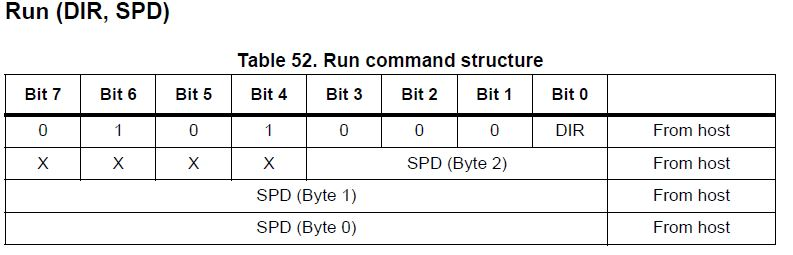
\includegraphics[width=10cm]{\EtPath/Bilder/command_example.JPG}
%        \caption{Beispiel eines Kommandos aus dem Datenblatt des l6480}
%        \label{fig:command}
%    \end{figure}
%    Der Treiber beinhaltet die Funktionen, welche die richtigen Bitfolgen über 
%    SPI an den L6480 senden. Fast alle dieser Funktionen wurden in 
%    Zusammenarbeit mit dem PREN-ET Team von Daniel Winz implementiert.  
%    \\\\
%    \textbf{Shell}\\
%    Für das Pneumatikventil und den Steppertreiber wurden Shellfunktionen 
%    implementiert. Erhält die Shell ein Kommando von der zentralen 
%    Recheneinheit, so wird die Eingabe ausgewertet und die entsprechende 
%    Shellfunktion ausgeführt. Die von der zentralen Recheneinheit geparsten 
%    Befehle sind:  
%    \begin{itemize}
%        \item l6480 run [f/r] [speed]
%        \item l6480 reset
%        \item l6480 softstop
%        \item l6480 hardstop
%        \item l6480 softhiz
%    \end{itemize}
%    für die Steuerung des Motor Controllers, sowie
%    \begin{itemize}
%        \item vent shoot
%    \end{itemize}
%    für die Steuerung des Pneumatikventils. 
%    \\\\
%    Der Befehl "l6480 run" lässt den Motor in Vorwärtsrichtung [f] oder 
%    Rückwärtsrichtung [r] mit der in [speed] definierten Geschwindigkeit 
%    drehen. "l6480 reset" konfiguriert den l6480 und bestromt den Motor, so 
%    dass dieser ein Haltemoment aufweist. Um den Motor ohne Haltemoment 
%    bewegen zu können, wird der Befehl "l6480 softhiz" verwendet, welcher die 
%    H-Brücke ausschaltet. 
    
